\documentclass[a4paper]{article}
\usepackage[utf8]{inputenc}
\usepackage{enumitem}
\usepackage{url}
\usepackage{hyperref}
\hypersetup{
    colorlinks=true,
    linkcolor=blue,
    filecolor=magenta,      
    urlcolor=cyan,
}
\usepackage{caption}
\usepackage{color}

\definecolor{lightgray}{rgb}{.9,.9,.9}
\definecolor{darkgray}{rgb}{.4,.4,.4}
\definecolor{purple}{rgb}{0.65, 0.12, 0.82}

\usepackage{listings}
\lstset{basicstyle=\ttfamily,
  showstringspaces=false,
  commentstyle=\color{red},
  keywordstyle=\color{blue},
  captionpos=b,
  breaklines=true,
  backgroundcolor=\color{lightgray},
  columns=fullflexible,
}
\lstdefinelanguage{javascript}{
  keywords={typeof, new, true, false, catch, function, return, null, catch, switch, var, if, in, while, do, else, case, break},
  keywordstyle=\color{blue}\bfseries,
  ndkeywords={class, export, boolean, throw, implements, import, this},
  ndkeywordstyle=\color{darkgray}\bfseries,
  identifierstyle=\color{black},
  sensitive=false,
  comment=[l]{//},
  morecomment=[s]{/*}{*/},
  commentstyle=\color{purple}\ttfamily,
  stringstyle=\color{red}\ttfamily,
  morestring=[b]',
  morestring=[b]"
}


% *** GRAPHICS RELATED PACKAGES ***
%\usepackage[pdftex]{graphicx}
\usepackage{graphicx}
%\usepackage[dvips]{graphicx}
% to place figures on a fixed position
\usepackage{float}

\usepackage[margin=1in]{geometry}

\title{Blockchains for Industrial IoT - a Tutorial \\ \large Cheat-sheet }

% \subtitle{Cheat sheet}

\author{Pal Varga and Ferenc Janky \\ Budapest University of Technology and Economics}


\date{v1.0 \\ 2019}

\begin{document}

\maketitle

\section{Login details}

\begin{itemize}
\item Demo environment: \url{https://blockchain.cnsm2019-tutorial.com/}
\begin{itemize}
\item username: \verb!user<X>! , where is \verb!<X>! is a number,  e.g.: \verb!user11!, the number allocation will happen at the time of starting the hands-on exercises
\item password: same as the username, e.g \verb!user11!
\end{itemize}
\item SSH access details:
\begin{itemize} 
\item host: blockchain.cnsm2019-tutorial.com
\item port: 2222
\item username: tutorial
\item password: cnsm2019
\end{itemize}
\end{itemize}

\section{Attaching to \emph{geth} node}

\begin{itemize}
\item SSH onto host specified above
\item Attach to \emph{geth} blockchain node by issueing command \verb!sudo ./admin/geth_attach!
\item the \emph{tutorial} user's password has to be given again
\end{itemize}

\section{Most frequently used \emph{geth} commands}

\begin{itemize}
\item the \emph{geth} console is a javascript REPL, any valid Javascript code is accepted. The commands below are actually \emph{web3} API calls, for all available commands see \url{https://web3js.readthedocs.io/en/v1.2.1/getting-started.html}

\item \verb!<variable name> = <expression>! assigns the result of expression  \verb!<expression>! to the variable named \verb!<variable>!, e.g. \verb!block34 = eth.getBlock(34)! that means assign the block object of block 34 to the variable named \verb!block34!


\item to define any custom function define a Javascript function and assign it to a variable:

\begin{lstlisting}[language=javascript]
myFunction = function(param1,param2,...) {
 // body of the function
}

// call the function with arguments
myFunction(arg1,arg2,...)
\end{lstlisting}

\item \verb!eth.accounts! an array of all accounts managed by this node

\item  After startup create this function : 
\begin{lstlisting}[language=javascript]
findAccount = function(addr){ return eth.accounts.filter(function(account){ return new RegExp(addr+".*","i").test(account) }) } \end{lstlisting}
this can be used to find an account starting with \verb!addr! e.g. \verb!findAccount("0x10db7")!

\item Note: scripts can be preloaded with the \verb!--preload path/to/script.js! argument when attaching to geth if needed

\item \verb!eth.getBalance(<account>)! for checking the balance of an account, where \verb!<account>! is a string literal having the value of the address of an Ethereum account or a deployed smart contract, e.g. \verb!eth.getBalance("0x9afeD102A10D54Cc6C0E5153752c69B4876A7419")!

\item \verb!web3.toWei(<value>,<dimension>)! for getting the equivalent value in \emph{Wei}s of the specified amount, where \verb!<value>! is a number literal and \verb!<dimension>! is a string literal having the name of a valid etherum metic, e.g. \verb!web3.toWei(3.14,"ether")!

\item \verb!eth.getBlock(<block Number>)! for getting a block's data specified by it's block number

\item \verb!eth.getTransaction(<transaction hash>)! for getting the transaction data specified by it's transaction hash

\item \verb!eth.getGasPrice(console.log)! will return the median \emph{gasPrice} based on the recently mined transaction or the default \emph{gasPrice} if there hasn't been any yet

\item \verb!eth.getTransactionCount(<account>,[<block specifier>])!, get the total transaction count for acount indicated by \verb!<account>!, optionally a block specifier can be supplied, e.g.: \\ \verb!eth.getTransactionCount("0x9afeD102A10D54Cc6C0E5153752c69B4876A7419","pending")! will get the transaction count for the given address including the pending transactions waiting in queue to be mined onto the blockchain

\item \verb!personal.signTransaction(<Transaction object>, <password>)! to sign a transaction with the senders private key represented by \verb!<Transaction object>! object where the sender's account has \verb!<password>! (string literal) as password, where a transaction has the following parameters

\begin{itemize}

\item \verb!from! : the sender's address

\item \verb!to! : the receiver's address

\item \verb!value! : the amount of \emph{Wei}s to be transferred to the receiver from the sender with this transaction

\item \verb!gas! : the amount of gas that can be consumed by the EVM for executing this transaction

\item \verb!gasPrice! : the price to be paid by the sender per units of gas consumed, the maximum price of the transaction will be \verb!value + gas*gasPrice!, if only fraction of the specified gas has been used by EVM, only the proportional price has to be paid while in contrast if the supplied gas was not enough the transaction will be reverted, but the gas price still has to be paid

\item \verb!nonce! : this is different from the block nonce in case of Proof-of-Work. This one indicates the total transaction count of the user in order to prevent double spending

\item \verb!data! : optional field, the additional data for this transaction, the code and data members are stored in this section of the transaction

\item Example:
\begin{lstlisting}[language=javascript]
signedTransaction = personal.signTransaction({
    from: "0x9afeD102A10D54Cc6C0E5153752c69B4876A7419",
    to: "0x3FecF304285303Fba1C34124889Ea1256e9BB0de",
    value: web3.toWei(1,"ether"),
    gas: 200000, 
    gasPrice: 10,
    nonce: 
    eth.getTransactionCount("0x9afeD102A10D54Cc6C0E5153752c69B4876A7419")
    },"user1" )
\end{lstlisting}

\end{itemize}

\item \verb!eth.sendRawTransaction(<Raw Transaction data>)! sends and execute the  provided transaction where \\ \verb!<Raw Transaction data>! is the raw transaction data in a hexadecimal string format, using the signed transaction object the raw transaction can be accessed by the \verb!raw! member variable, e.g.: \\ \verb!eth.sendRawTransaction(signedTransaction.raw)!

\end{itemize}


\section{PowerBid game details}

By playing this game we'll deploy smart contracts and also interact with each other's contract through its well-defined API. This game realizes a sell auction where the subject of the auction is electrical power. There are 2 roles:
\begin{itemize}
\item Consumer , who creates the contract
\item Supplier, who bids on the Consumer's contract
\end{itemize}

The game can be split up to the following main phases (a detailed state diagram is shown on Figure \ref{fig:State-diagram-powerbid}):

\begin{enumerate}
    \item Auction Phase, where the suppliers participate in the sell auction
    \item Consumption Phase, where the consumer consumes the power paid and requested
    \item Withdraw Phase, where the consumer can withdraw his gain (that is the difference between the max. price and the best price) and the supplier can withdraw the funds from the contract
\end{enumerate}


\begin{figure}[H]
    \centering
    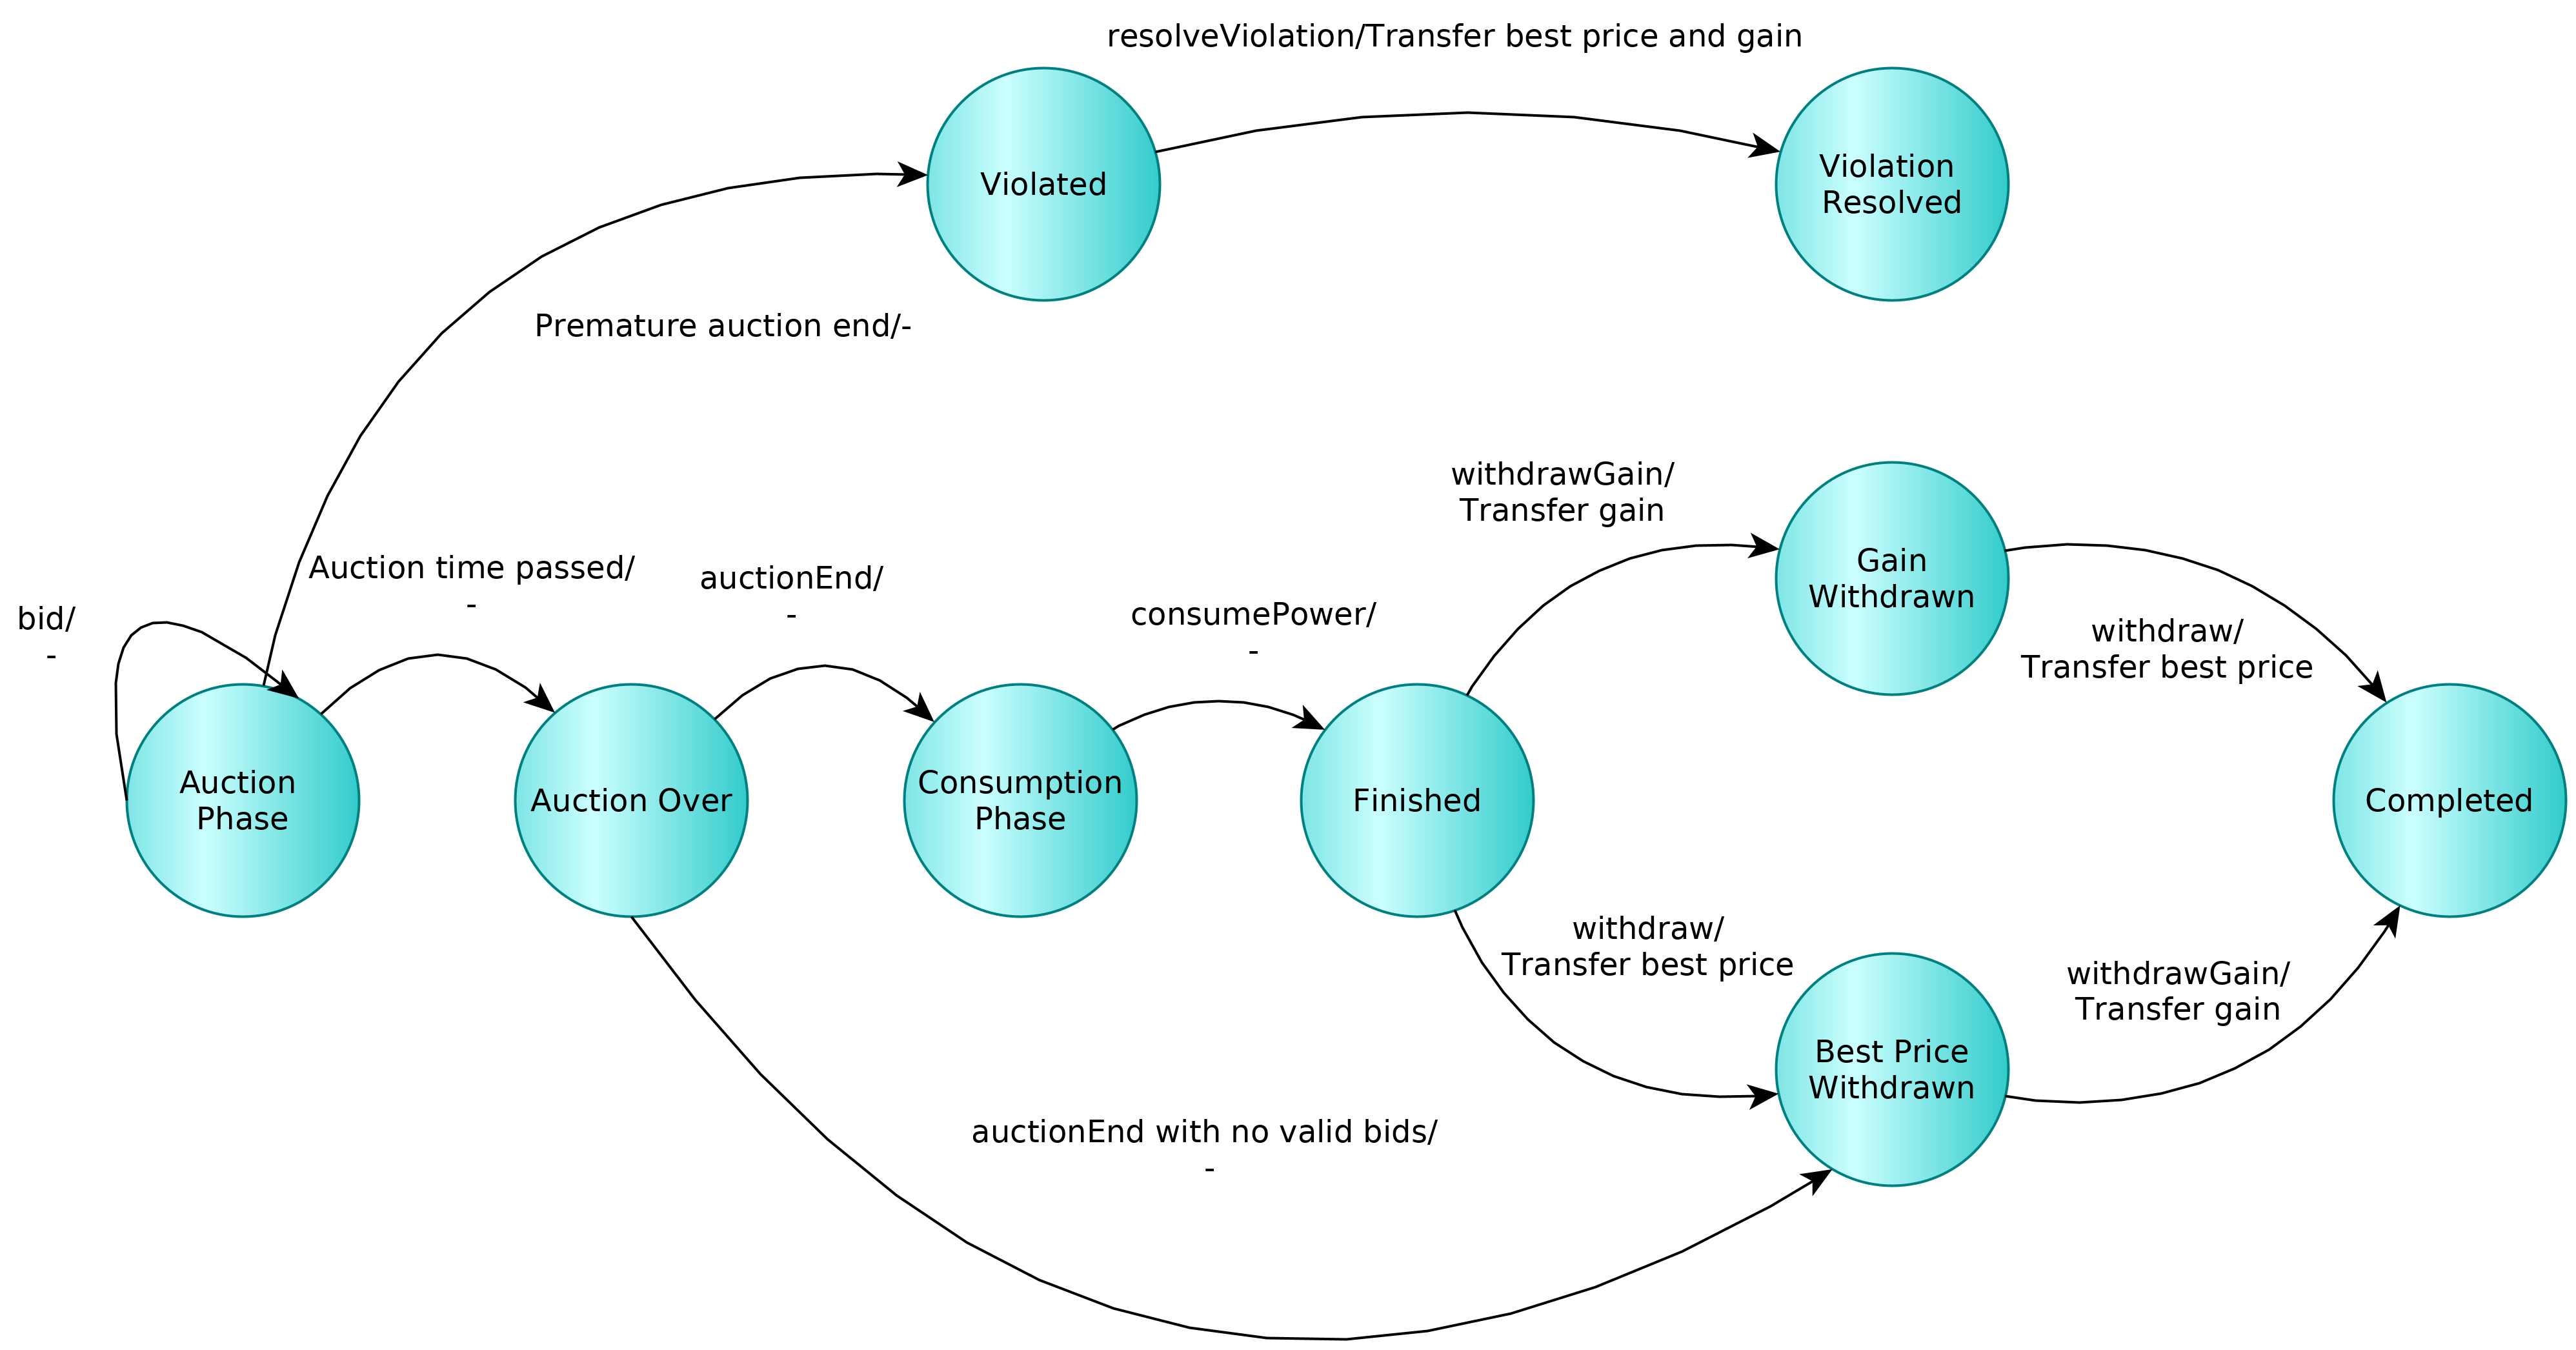
\includegraphics[width=0.9\textwidth]{figures/state_diagram.png}
    \caption{The state diagram of the PowerBid smart contract}
    \label{fig:State-diagram-powerbid}
\end{figure}

\subsection{Game-play summary}

The high-level game-play for the two different roles can be summarized as:
\begin{itemize}
    \item Consumer role:
    \begin{enumerate}
        \item Deploy contract after specifying the constructor parameters
        \item Monitor the sell auction until the auction is ongoing.
        \item Consume the power (virtually, calling the \emph{'consumePower'} API by pressing the corresponding button)
        \item withdraw gains (Max. price - best price)
        \item evaluate relative gain
    \end{enumerate}
    \item Producer/Supplier role:
    \begin{enumerate}
        \item Bid on the deployed Smart contracts
        \item monitor bid state based on the visual feedback and/or polling the contracts
        \item place further bids as desired
        \item wait for consumer to consume the power
        \item withdraw the price amount from the contracts that has been win by the user
        \item evaluate relative gain
    \end{enumerate}
\end{itemize}

\subsection{Typical values to use}
\begin{itemize}
    \item \emph{gasPrice} : set to 10 Wei, otherwise the balance could drain quickly
    \item Consumer role (contract creation):
    \begin{itemize}
        \item \emph{value}: somewhere betwee 900-1000 finneys
        \item \emph{auctionPeriodSeconds}: 300 (seconds) so that will be enough time for bidding
        \item \emph{consumptionPeriodSeconds}: 60 (seconds) is enough
        \item \emph{requiredEnergy}: set it to 100000
    \end{itemize}
    \item Supplier role:
    \begin{itemize}
        \item when bidding don't go lower than 80\% of the \emph{maxPrice}
    \end{itemize}
\end{itemize}

\section{Implement a number guessing game}

The game participants are guessing numbers. The winner is who choose the smallest number. If a number has been chosen by more than 1 person it is not considered as a valid guess. 1 person can only guess once. The creator offers a prize that (greater than 0 Wei) is to be won by the winner. If at the end of the game there are no valid guesses the creator is considered the winner. Only the winner must be able to withdraw the prize. At construction time the owner should be able to specify the total number of guesses that will limit the number of individuals who are able to play the game. The prize mustn't be possible to be withdrawn before the game ends. The results should only be possible to be queried through the programmatic API when the game is over. 

The contract template can be downloaded from: \url{https://raw.githubusercontent.com/fecjanky/iot_sc_tutorial/master/src/NumberGuessing_template.sol}

\emph{Remix IDE}:\url{http://remix.ethereum.org/}

\section{Demo environment/source code info}

If there's a need for further experimentation with this blockchain demo environment its Docker image can be pulled from DockerHub and run by 

\begin{lstlisting}[language=bash]
docker pull fecjanky/iot_sc_tutorial:latest
docker run -p 2222:22 -p 80:80 -p 443:443 fecjanky/iot_sc_tutorial:latest
\end{lstlisting}

NB.: port bindings can be changed freely

The source code can be obtained from : \url{https://github.com/fecjanky/iot_sc_tutorial}

\end{document}